\documentclass{report}
\usepackage{pdfpages}
\usepackage{pgf,tikz}
\usetikzlibrary{arrows}

\begin{document}
\thispagestyle{empty}
\begin{center}
{\Huge Transactions\\ in\\[.2in] \textbf{Euclidean Geometry}}
\vspace{1in}

\begin{figure}[h!]
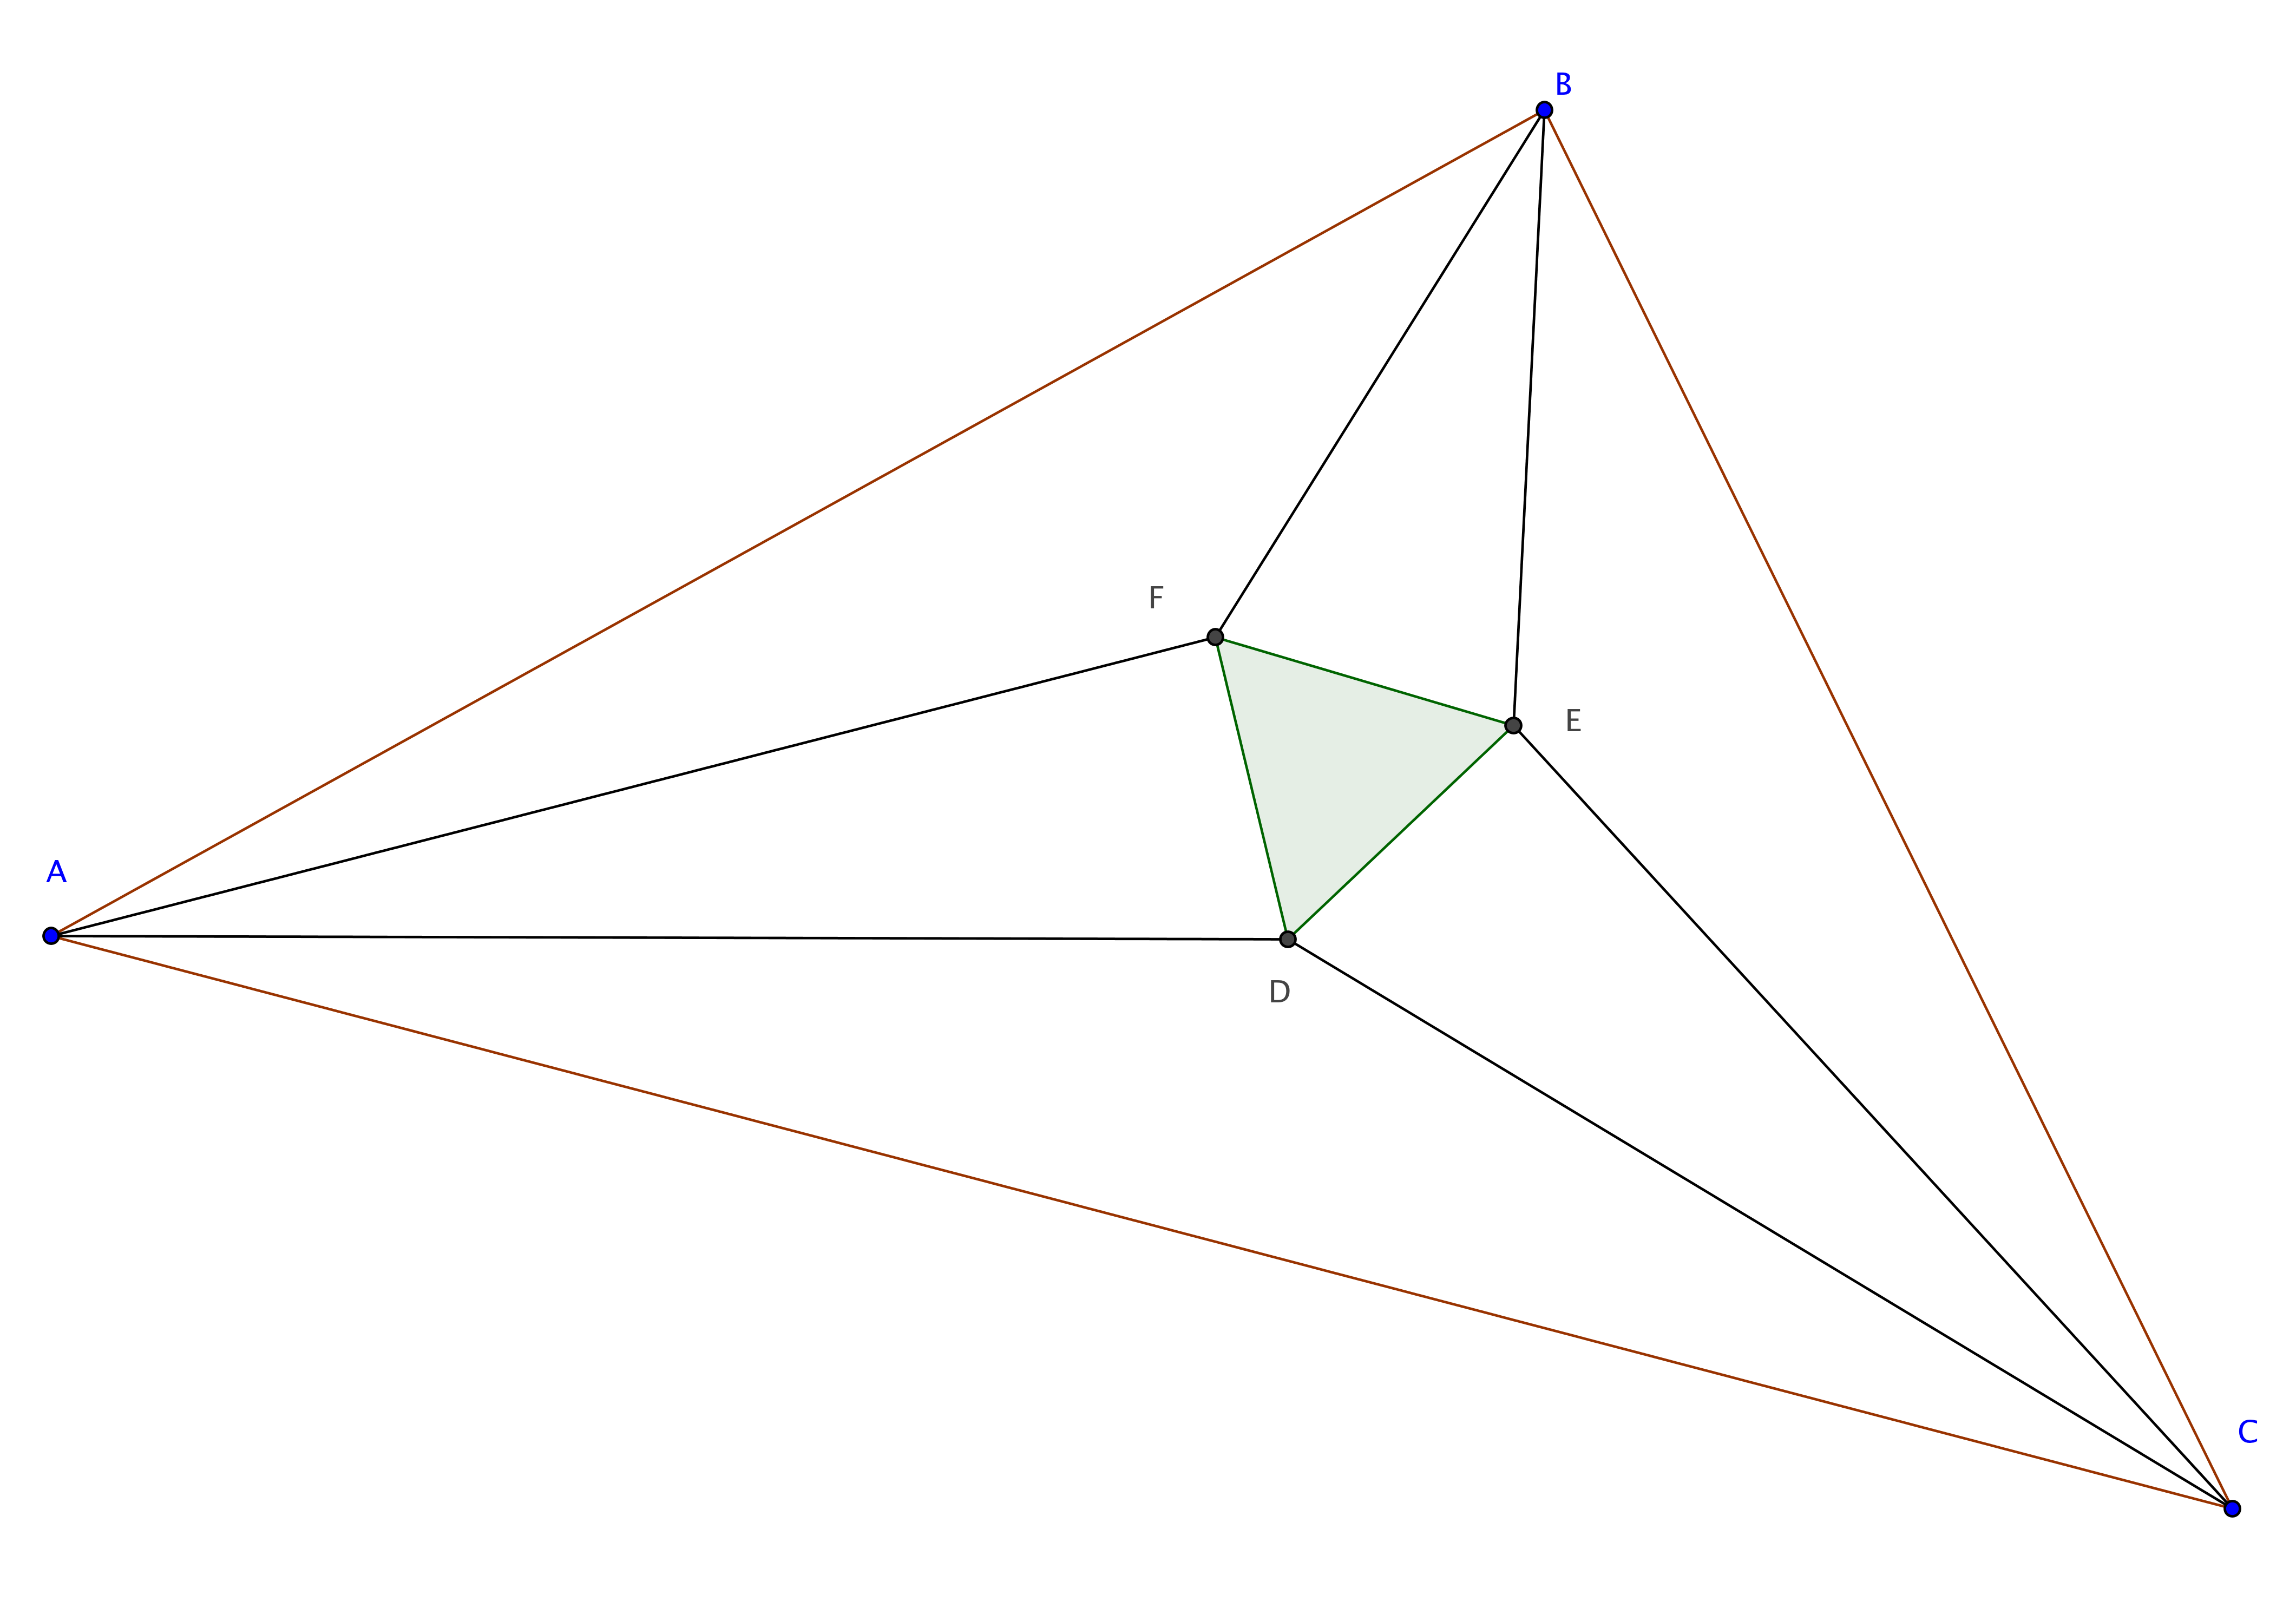
\includegraphics[width=1.1\textwidth]{cover-image.png}
\end{figure}

\vspace{1in}

{\Huge Volume 2021F Issue \# 0}
\end{center}

\clearpage

\center \Large \textbf{Table of Contents}\\[.5in]
\normalsize
\begin{tabular}{lr}
\textbf{Title} & \textbf{Author}\\[.25in]
\emph{The Symmetric Nature of Triangles} & W.W. Rouse Ball \\[.25in]
\emph{Relocating a Segment} & Theron J Hitchman \\[.25in]
\emph{An Inequality for an Exterior Angle of a Triangle} & Theron J Hitchman \\[.25in]
%\emph{Convex or Non-Convex Polygons} & Staci Schmeling \& \\
%				& Mackenzie Mitchell \\[.25in]
%\emph{Fixing Euclid Proposition 7} & Tessa Cohen \& \\
%									& Erica Schultz \\[.25in]
%\emph{A Regular Rhombus is a Square} & Staci Schmeling \\[.25in]
%\emph{Pentagon Regularity Given Certain Angles} & Danielle Maus \\[.25in]
%\emph{Angle Bisectors of a Triangle are Concurrent} & Taryn Van Ryswyk \\[.25in]
%\emph{Tangent Line Congruency} & Christopher Merck\\[.25in]
%\emph{SSS Theorem and Circle Intersections} & Christopher Merck\\[.25in]
%\emph{Cyclic Quadrilaterals} & Danielle Maus \\[.25in]
%\emph{A Circle Contains the Sum of Four Right Angles} & Taryn Van Ryswyk \\
\end{tabular}

\includepdf[pages=-]{Ball-Fallacy.pdf}
\includepdf[pages=-]{example-wk02.pdf}
\includepdf[pages=-]{example-wk03.pdf}
%\includepdf[pages=-]{4.pdf}
%\includepdf[pages=-]{5.pdf}
%\includepdf[pages=-]{6.pdf}
%\includepdf[pages=-]{7.pdf}
%\includepdf[pages=-]{8.pdf}
%\includepdf[pages=-]{9.pdf}
%\includepdf[pages=-]{10.pdf}
%\includepdf[pages=-]{11.pdf}
%\includepdf[pages=-]{12.pdf}

\end{document}